\section{Results}
\label{sec:results}

All values in this section were generated from the locked V1 final artifact. The
evaluation contains 4,000 fixed verification trials (200 genuine and 3,800
impostor) in each of 15 conditions. The 20 identity labels denote public
biometric instances; they are not asserted to be independent people. We
therefore report bounded benchmark point estimates and do not attach
person-population confidence intervals or hypothesis tests.

\subsection{Q1: contribution of deep fusion}

Table~\ref{tab:v1-clean-results} and Figure~\ref{fig:v1-clean-eer} summarize the
clean condition. Classical feature concatenation (C4) achieved the lowest
ROCCH-EER, 0.2115, compared with 0.3097 for the best unimodal system (U-FP), an
absolute reduction of 0.0982. Equal score fusion (C1) did not improve on U-FP
(0.3105 versus 0.3097).

The best deep family was feature fusion D2 (0.2865), but it remained 0.0750
above the matched classical feature method C4. Within the score stratum, D1
(0.3098) did not improve over C2 (0.3088). The quality-aware deep gate D3S
(0.3104) was slightly lower than C5 (0.3136), by 0.0032, but both were worse
than C4. Thus V1 supports a benefit for multimodal classical feature fusion on
this benchmark, not a general benefit for deep fusion.

\begin{table*}[t]
\centering
\small
\caption{Clean-condition V1 results. Lower is better for EER and calibration losses; higher is better for AUC.}
\label{tab:v1-clean-results}
\begin{tabular}{lrrrrr}
\toprule
System & ROCCH-EER & AUC & $C_{llr}$ & Brier & ECE \\
\midrule
U-FP & 0.3097 & 0.7453 & 0.9585 & 0.2207 & 0.4180 \\
U-FV & 0.3441 & 0.7172 & 0.9690 & 0.2258 & 0.4237 \\
C1 & 0.3105 & 0.7704 & 1.3030 & 0.0762 & 0.1138 \\
C2 & 0.3088 & 0.7732 & 1.3454 & 0.0747 & 0.1071 \\
C3 & 0.3093 & 0.7685 & 1.4290 & 0.0764 & 0.1100 \\
C4 & 0.2115 & 0.8632 & 0.7758 & 0.0727 & 0.1690 \\
C5 & 0.3136 & 0.7557 & 1.5820 & 0.0752 & 0.1032 \\
D1 & 0.3098 & 0.7625 & 1.0379 & 0.0880 & 0.1536 \\
D2 & 0.2865 & 0.7904 & 0.9673 & 0.1482 & 0.1990 \\
D3S & 0.3104 & 0.7644 & 1.2842 & 0.0789 & 0.1196 \\
\bottomrule
\end{tabular}
\end{table*}

\begin{figure*}[t]
\centering
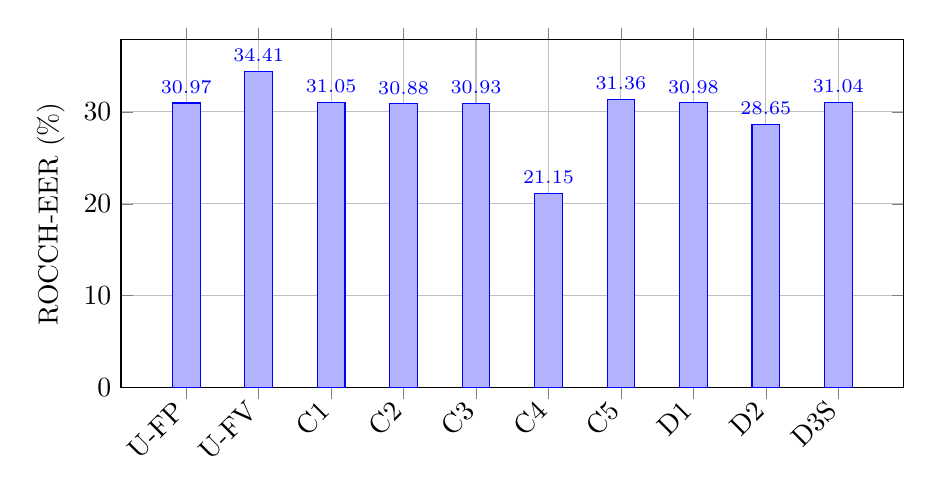
\begin{tikzpicture}
\begin{axis}[ybar, width=0.95\textwidth, height=6cm, ymin=0, ylabel={ROCCH-EER (\%)}, symbolic x coords={U-FP,U-FV,C1,C2,C3,C4,C5,D1,D2,D3S}, xtick=data, x tick label style={rotate=45,anchor=east}, nodes near coords, nodes near coords style={font=\scriptsize}, grid=major]
\addplot coordinates {(U-FP,30.969136) (U-FV,34.406793) (C1,31.053879) (C2,30.876043) (C3,30.928887) (C4,21.146749) (C5,31.362543) (D1,30.983505) (D2,28.645278) (D3S,31.040809)};
\end{axis}
\end{tikzpicture}
\caption{Clean-condition discrimination on the locked V1 final trials. Lower is better.}
\label{fig:v1-clean-eer}
\end{figure*}


\subsection{Q2: performance--robustness--calibration--cost trade-off}

The locked four-dimensional point-estimate Pareto analysis identifies C1, C2,
C4, D1, and D2 as non-dominated (Table~\ref{tab:v1-q2-pareto}). C4 combines the
lowest clean error with the strongest condition-wise discrimination, but its
fusion-only median latency was 2.930~ms. D2 required 1.928~ms and 139,456
trainable parameters; it had the smallest mean stress ROCCH-EER loss (0.0030)
among the reported families, but worse clean error than C4. Low-capacity score
systems remained on the frontier because of their much smaller latencies.
Consequently no single deep family is the unqualified best trade-off, and no
point-estimate frontier membership is interpreted as uncertainty-supported
dominance.

\begin{table*}[t]
\centering
\small
\caption{Locked four-dimensional Q2 point-estimate Pareto analysis.}
\label{tab:v1-q2-pareto}
\begin{tabular}{lrrrrc}
\toprule
System & EER & Robustness loss & $C_{llr}$ & Latency (ms) & Pareto \\
\midrule
C1 & 0.3105 & 0.0140 & 1.3030 & 0.043 & yes \\
C2 & 0.3088 & 0.0149 & 1.3454 & 0.029 & yes \\
C3 & 0.3093 & 0.0156 & 1.4290 & 0.105 & no \\
C4 & 0.2115 & 0.0364 & 0.7758 & 2.930 & yes \\
C5 & 0.3136 & 0.0219 & 1.5820 & 0.085 & no \\
D1 & 0.3098 & 0.0138 & 1.0379 & 0.077 & yes \\
D2 & 0.2865 & 0.0030 & 0.9673 & 1.928 & yes \\
D3S & 0.3104 & 0.0164 & 1.2842 & 0.224 & no \\
\bottomrule
\end{tabular}
\end{table*}

\begin{figure}[t]
\centering
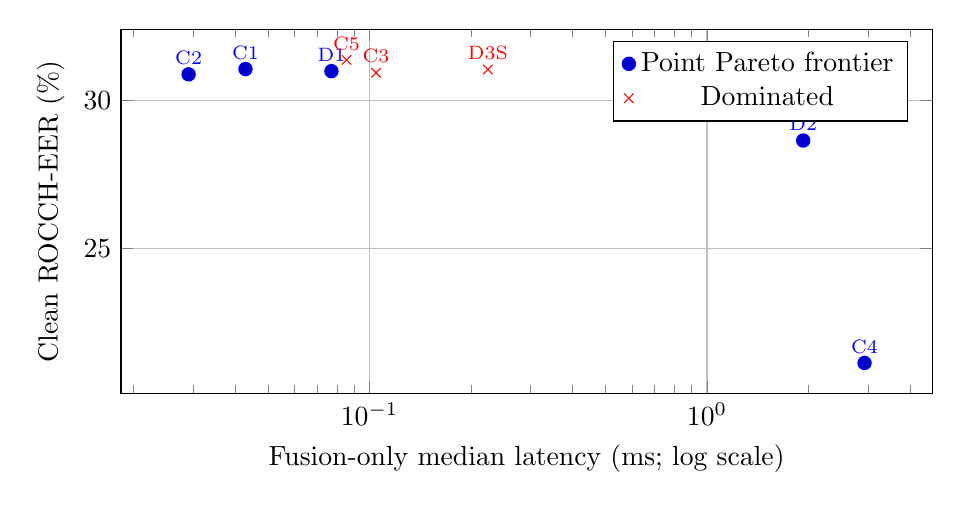
\begin{tikzpicture}
\begin{axis}[width=0.98\columnwidth,height=6.2cm,xmode=log,xlabel={Fusion-only median latency (ms; log scale)},ylabel={Clean ROCCH-EER (\%)},grid=major,legend pos=north east,point meta=explicit symbolic,nodes near coords,nodes near coords style={font=\scriptsize,anchor=south}]
\addplot+[only marks,mark=*,mark size=2.4pt] coordinates {(0.042879000,31.053879) [C1] (0.029089000,30.876043) [C2] (2.930127000,21.146749) [C4] (0.077098000,30.983505) [D1] (1.928308500,28.645278) [D2]};
\addlegendentry{Point Pareto frontier}
\addplot+[only marks,mark=x,mark size=2.4pt] coordinates {(0.104513500,30.928887) [C3] (0.085443500,31.362543) [C5] (0.224206000,31.040809) [D3S]};
\addlegendentry{Dominated}
\end{axis}
\end{tikzpicture}
\caption{Two visible Q2 dimensions. Pareto membership is computed from all four locked dimensions, including robustness loss and $C_{llr}$.}
\label{fig:v1-q2-pareto}
\end{figure}


\subsection{Q3: degradation and modality absence}

C4 had the lowest ROCCH-EER in clean data and in every one of the 12 locked
blur/contrast conditions. Rankings below the winner did change: Kendall's
$\tau_b$ against the clean ranking ranged from 0.2143 to 0.8571 across those
conditions, with 2--11 pairwise reversals. The most severe fingerprint blur
produced both the lowest agreement ($\tau_b=0.2143$) and 11 reversals.

Under the frozen M0 missing-modality policy, every fusion family falls back to
the same available unimodal evidence. All eight fusion methods therefore tie at
0.3097 when finger vein is missing and at 0.3441 when fingerprint is missing.
Kendall's $\tau_b$ is mathematically undefined for these all-tie rankings and is
stored as JSON \texttt{null}; the serialized row order is only a deterministic
tie break. These conditions validate the declared fallback, not a learned
missing-modality advantage.

\begin{figure*}[t]
\centering
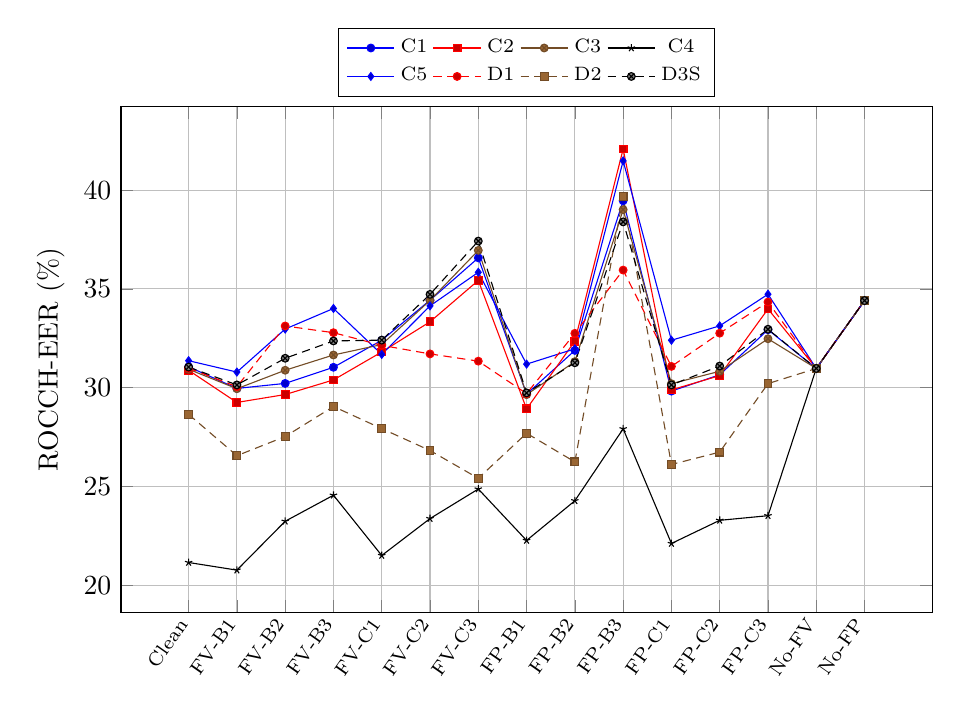
\begin{tikzpicture}
\begin{axis}[width=0.98\textwidth,height=8cm,ylabel={ROCCH-EER (\%)},symbolic x coords={Clean,FV-B1,FV-B2,FV-B3,FV-C1,FV-C2,FV-C3,FP-B1,FP-B2,FP-B3,FP-C1,FP-C2,FP-C3,No-FV,No-FP},xtick=data,x tick label style={rotate=55,anchor=east,font=\scriptsize},legend columns=4,legend style={at={(0.5,1.02)},anchor=south,font=\scriptsize},grid=major,mark size=1.4pt]
\addplot coordinates {(Clean,31.053879) (FV-B1,29.960018) (FV-B2,30.212777) (FV-B3,31.029605) (FV-C1,32.397720) (FV-C2,34.425000) (FV-C3,36.568695) (FP-B1,29.670781) (FP-B2,31.883612) (FP-B3,39.461538) (FP-C1,29.823362) (FP-C2,30.649566) (FP-C3,32.931398) (No-FV,30.969136) (No-FP,34.406793)};
\addlegendentry{C1}
\addplot coordinates {(Clean,30.876043) (FV-B1,29.250000) (FV-B2,29.649671) (FV-B3,30.388634) (FV-C1,31.804301) (FV-C2,33.332711) (FV-C3,35.426606) (FP-B1,28.922035) (FP-B2,32.352636) (FP-B3,42.080590) (FP-C1,29.886354) (FP-C2,30.606757) (FP-C3,33.980130) (No-FV,30.969136) (No-FP,34.406793)};
\addlegendentry{C2}
\addplot coordinates {(Clean,30.928887) (FV-B1,29.943925) (FV-B2,30.880000) (FV-B3,31.651703) (FV-C1,32.181934) (FV-C2,34.414088) (FV-C3,36.946803) (FP-B1,29.644362) (FP-B2,31.315500) (FP-B3,39.010761) (FP-C1,30.198800) (FP-C2,30.827131) (FP-C3,32.472661) (No-FV,30.969136) (No-FP,34.406793)};
\addlegendentry{C3}
\addplot coordinates {(Clean,21.146749) (FV-B1,20.759950) (FV-B2,23.234456) (FV-B3,24.553130) (FV-C1,21.501866) (FV-C2,23.370130) (FV-C3,24.867347) (FP-B1,22.262861) (FP-B2,24.272131) (FP-B3,27.913994) (FP-C1,22.109799) (FP-C2,23.281337) (FP-C3,23.515957) (No-FV,30.969136) (No-FP,34.406793)};
\addlegendentry{C4}
\addplot coordinates {(Clean,31.362543) (FV-B1,30.786874) (FV-B2,32.965116) (FV-B3,34.006444) (FV-C1,31.679598) (FV-C2,34.137066) (FV-C3,35.838422) (FP-B1,31.189003) (FP-B2,31.963872) (FP-B3,41.478361) (FP-C1,32.397297) (FP-C2,33.126284) (FP-C3,34.727525) (No-FV,30.969136) (No-FP,34.406793)};
\addlegendentry{C5}
\addplot coordinates {(Clean,30.983505) (FV-B1,30.045802) (FV-B2,33.120038) (FV-B3,32.780612) (FV-C1,32.138776) (FV-C2,31.706738) (FV-C3,31.340474) (FP-B1,29.696970) (FP-B2,32.748349) (FP-B3,35.950374) (FP-C1,31.074054) (FP-C2,32.756329) (FP-C3,34.333406) (No-FV,30.969136) (No-FP,34.406793)};
\addlegendentry{D1}
\addplot coordinates {(Clean,28.645278) (FV-B1,26.553756) (FV-B2,27.523055) (FV-B3,29.043707) (FV-C1,27.924855) (FV-C2,26.815068) (FV-C3,25.408213) (FP-B1,27.690174) (FP-B2,26.238938) (FP-B3,39.675145) (FP-C1,26.107994) (FP-C2,26.735614) (FP-C3,30.203849) (No-FV,30.969136) (No-FP,34.406793)};
\addlegendentry{D2}
\addplot coordinates {(Clean,31.040809) (FV-B1,30.136111) (FV-B2,31.486081) (FV-B3,32.362559) (FV-C1,32.404762) (FV-C2,34.721342) (FV-C3,37.418704) (FP-B1,29.732789) (FP-B2,31.256983) (FP-B3,38.391185) (FP-C1,30.137342) (FP-C2,31.093681) (FP-C3,32.955379) (No-FV,30.969136) (No-FP,34.406793)};
\addlegendentry{D3S}
\end{axis}
\end{tikzpicture}
\caption{Condition-wise fusion-system discrimination using the clean calibrator transfer policy. Missing-modality ties follow the frozen M0 fallback.}
\label{fig:v1-q3-conditionwise}
\end{figure*}


\subsection{Calibration transfer}

Clean-condition affine calibrators were fitted only on the calibration split
and transferred unchanged to final conditions. Matching-condition
recalibration is reported as a diagnostic secondary analysis and does not
replace the primary transfer result. Figure~\ref{fig:v1-calibration-transfer}
shows that calibration behavior depends strongly on this choice; discrimination
metrics alone are therefore not used to claim calibration improvement.

\begin{figure*}[t]
\centering
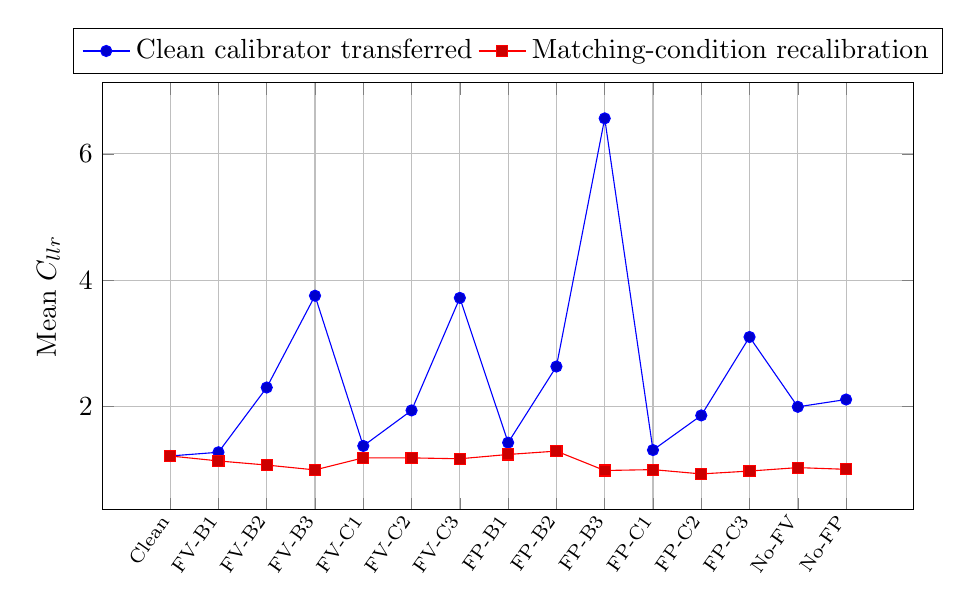
\begin{tikzpicture}
\begin{axis}[width=0.98\textwidth,height=7cm,ylabel={Mean $C_{llr}$},symbolic x coords={Clean,FV-B1,FV-B2,FV-B3,FV-C1,FV-C2,FV-C3,FP-B1,FP-B2,FP-B3,FP-C1,FP-C2,FP-C3,No-FV,No-FP},xtick=data,x tick label style={rotate=55,anchor=east,font=\scriptsize},grid=major,legend style={at={(0.5,1.02)},anchor=south,legend columns=2}]
\addplot coordinates {(Clean,1.215567) (FV-B1,1.274317) (FV-B2,2.299923) (FV-B3,3.753464) (FV-C1,1.374586) (FV-C2,1.937225) (FV-C3,3.719038) (FP-B1,1.426603) (FP-B2,2.632303) (FP-B3,6.562104) (FP-C1,1.309000) (FP-C2,1.857931) (FP-C3,3.099732) (No-FV,1.993928) (No-FP,2.109808)};
\addlegendentry{Clean calibrator transferred}
\addplot coordinates {(Clean,1.215567) (FV-B1,1.136864) (FV-B2,1.071614) (FV-B3,0.994705) (FV-C1,1.185755) (FV-C2,1.185091) (FV-C3,1.171241) (FP-B1,1.239374) (FP-B2,1.292585) (FP-B3,0.985440) (FP-C1,0.999372) (FP-C2,0.931326) (FP-C3,0.976730) (No-FV,1.031250) (No-FP,1.004154)};
\addlegendentry{Matching-condition recalibration}
\end{axis}
\end{tikzpicture}
\caption{Calibration robustness over the eight fusion systems. Matching-condition recalibration is diagnostic and does not replace the primary clean-calibrator transfer result.}
\label{fig:v1-calibration-transfer}
\end{figure*}

